\documentclass[a4paper,12pt]{scrartcl}
\usepackage[ngerman]{babel}
\usepackage{graphicx} %BIlder einbinden
\usepackage{amsfonts,amsmath,amssymb,amsthm} %erweiterte Mathe-Zeichen
\usepackage{mathtools}
\usepackage[utf8]{inputenc} %Umlaute & Co
\usepackage{fancyhdr}
\usepackage{forloop}
\usepackage{ifthen}
\usepackage{courier}
\usepackage{blkarray}
\usepackage{listings}
\usepackage{tikz}
\usepackage{color}
\usepackage{cancel}
\usepackage{enumerate}
\pagestyle{fancy}
\usepackage{mathtools}
\usepackage{ marvosym }
\usepackage[]{algorithm2e}
\usepackage{pgfplots}
\usepackage{listings}
\usepackage[normalem]{ulem} % [normalem] to set \emph{} to default behaviour (italic instead of underlining)
\usepackage{mdsymbol}
\DeclarePairedDelimiter{\ceil}{\lceil}{\rceil}
\DeclarePairedDelimiter{\floor}{\lfloor}{\rfloor}
\fancyhf{}
\rhead{Informatik II Thorsten Gruscht}
\lhead{Alle Vorlesungen}
\newcommand{\linie}{\noindent\makebox[\linewidth]{\rule{\paperwidth}{0.4pt}}}
\newcommand{\auf}{\textless}
\newcommand{\zu}{\textgreater}
\newcommand{\eval}{$\longrightsquigarrow$}
\renewcommand{\i}{\item}
\renewcommand{\t}{\text}
\begin{document}
\section*{14.4.2015}
\section*{Scheme}
\underline{A}usdr\"ucke , \underline{A}uswertung und \underline{A}bstraktion\\
\subsection*{Dr Racket}
\fbox{
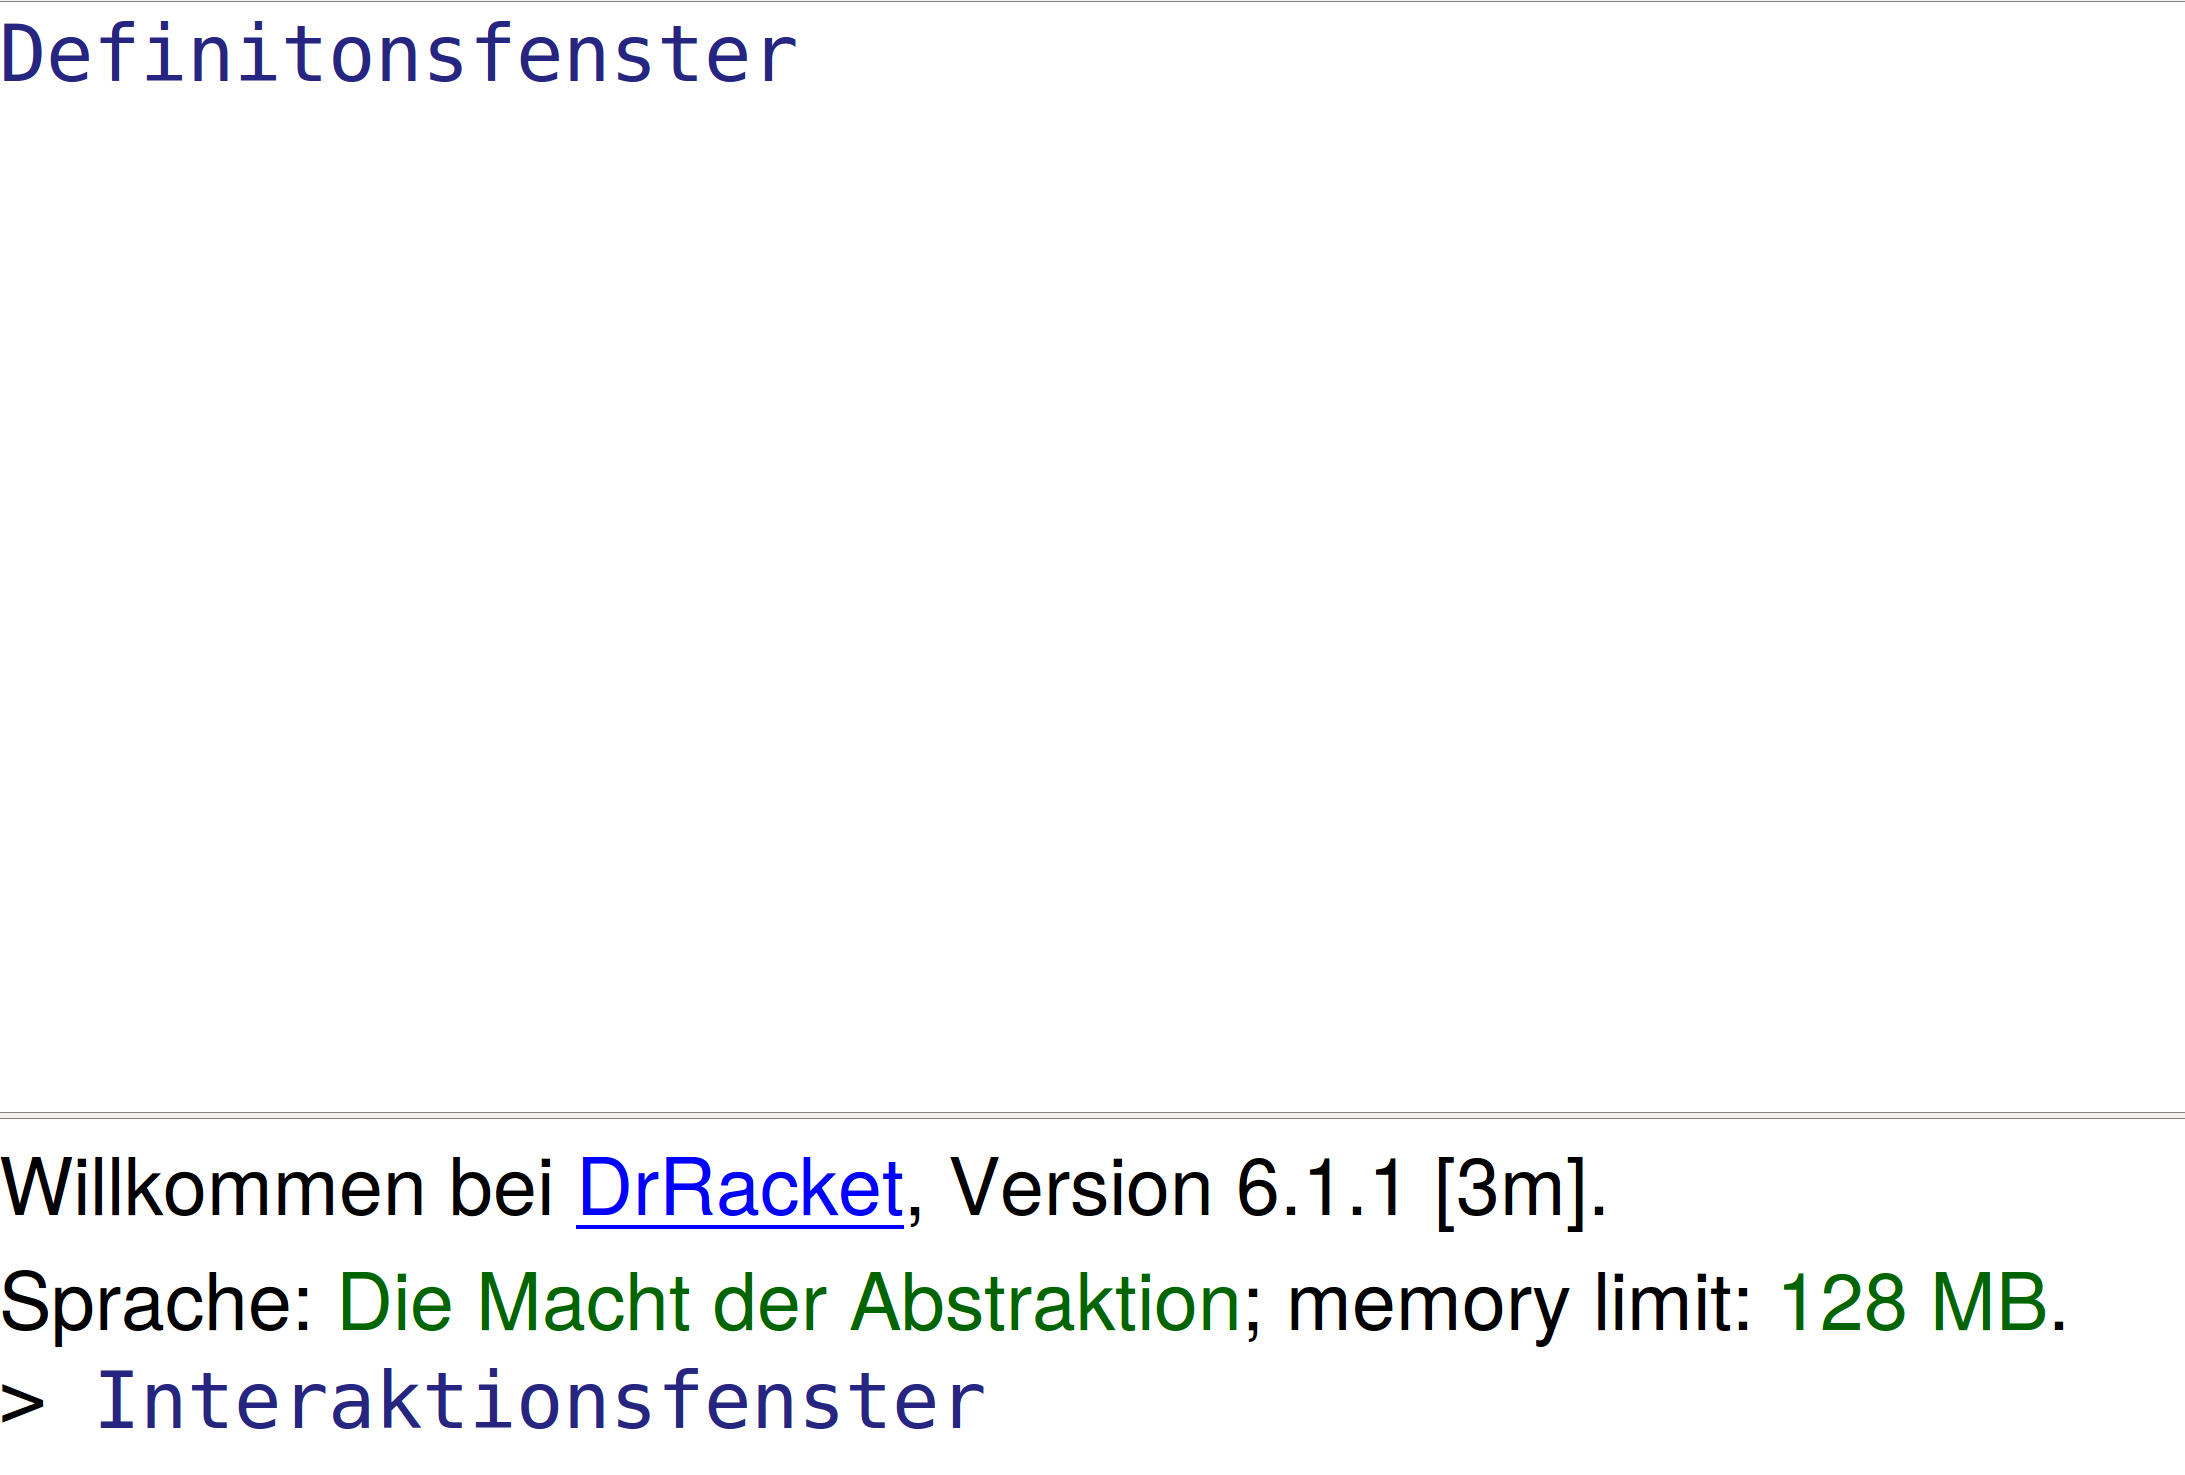
\includegraphics[scale=0.15]{drracket}}\\
Die Anwendung von Funktionen wird in Scheme ausschlie\ss lich in Pr\"afixnotation durchgef\"uhrt
\bigskip\\
\begin{center}
\begin{tabular}{c|c}
Mathematik & Scheme \\
\hline
$44-2$ & $(- $44 2)\\
$f(x,y)$ & (f x y)\\
$\sqrt{81}$ & (sqrt 81)\\
$9^2$ & (expt 92)\\
$3!$ & (! 3)\\
\end{tabular}\\
Allgemein: (\textless funktion\textgreater \textless argument1\textgreater \textless argument2\textgreater \ldots)
\end{center}
(+ 40 2) und (odd? 42) sind Beispiele f\"ur \underline{Ausdr\"ucke}, die bei \underline{Auswertung} einen Wert liefern.\\
(Notation: \eval)\\
(+ 40 2) $\underbrace{\longrightsquigarrow}_{Reduktion}$ 42\\
(odd? 42) \eval \#f
\bigskip\\
Interaktionsfenster:\hspace*{2.5cm} $\underbrace{Read \rightarrow Eval \rightarrow Print \rightarrow Loop}_{REPL}$\\
\bigskip\\
\underline{Literale} sethen f\"ur einen konstanten Wert (auch: \underline{Konstante}) und sind nicht weiter reduzierbar.\\
\begin{center}
\begin{tabular}{ccc}
Literal &  & Sorte,Typ\\
\hline
\#f ,\#t & (true, false, Wahrheitswert) & boolean\\
"x" & (Zeichenketten) & String\\
0 1904 42 $-2$ & (ganze Zahl) & Integer\\
0.42 3.14159 & (Flie\ss kommazahl) & real\\
1\textbackslash 2, 3\textbackslash 4, -1\textbackslash 10 & (rationale Zahlen) & rational\\

\includegraphics[scale=0.2]{Darth_Vader} & (Bilder) & image

\end{tabular}
\end{center}



\section*{16.4.2015}

Auswertung \underline{zusammengesetzter Ausdr\"ucke} in mehreren Schritten (Steps), von ``innen nach au\ss en``, bis keine Reduktion mehr m\"oglich ist.\\
\begin{lstlisting}
(+ ( @\uwave{(+ 20 20)}@ (+ 1 1)) @\eval@ (+ 40 @\uwave{(+ 1 1)}@ @\eval@ (+ 40 2) @\eval@  42 
\end{lstlisting}
\rackett{Arithmetik mit Flie\ss kommazahlen}{\textbf{Achtung:} Scheme rundet bei Arithmetik mit Flie\ss kommazahlen (interne Darstellung ist binär}{Grundlagen}{4}{17}
Ein Wert kann an einen \underline{Namen} (auch \underline{Identifier}) gebunden werden, durch \\
\lstinline!(define <id> <e>)! \hspace*{1.5cm} \auf id\zu Identifier \ \auf e\zu Ausdruck\\
Erlaubte konsistente Wiederverwendung, dient der Selbstdokumentation von Programmen\\
\textbf{\underline{Achtung:}} Dies ist eine sogenannte Spezialform und kein Ausdruck. Insbesondere besitzt diese Spezialform \underline{keinen} Wert, sondern einen Effekt Name \auf id\zu \ wird an den \underline{Wert} von \auf e\zu \ gebunden. \\
Namen k\"onnen in Scheme beliebig gewählt werden, solange
\begin{enumerate}
\item[(1)] die Zeichen ( ) $[$ $]$ $\{ \}$ `` , ` ` ; \# $\mid$ \textbackslash nicht vorkommen
\item[(2)] dieser nicht einem numerischen Literal gleicht.
\item[(3)] kein Whitespace (Leerzeichen, Tabulator, Return) enthalten ist.
\end{enumerate}
Beispiel: euro$\rightarrow$US\$\\
\underline{\textbf{Achtung:}} Gro\ss-\textbackslash Kleinschreibung ist irrelevant.
\bigskip\\
\lstinputlisting[frame=single,caption={[Schlüsselwort define]Bindung von Werten an Namen},firstline=19,lastline=24]{Grundlagen.rkt}
Eine \underline{lambda-Abstraktion} (auch Funktion, Prozedur) erlaubt die Formatierung von Ausrdr\"ucken, in denen mittels \underline{Parametern} von konkreten Werten abstrahiert wird.\\
\lstinline[literate=]!(lambda (<p1><p2>...) <e>!\\
\auf e\zu Rumpf: enth\"alt Vorkommen der Parameter \auf $p_n$\zu\\
(lambda($\ldots$)) ist eine Spezialform. Wert der lambda-Abstraktion ist \#\auf procedure\zu\\.
\underline{Anwendung} (auch Application) des lambda-Aufrufs f\"uhrt zur Ersetzung aller Vorkommen der Parameter im Rumpf durch die angegebenen \uline{Argumente}.\\
\lstinputlisting[frame=single,caption={[Lambda Abstraktion] Lambda-Abstraktion},firstline=26,lastline=34]{Grundlagen.rkt}
\lstinline!(lambda (days) (* days (* 155!\lstinline! minutes-in-a-day))) 365)! \eval\\
\lstinline!(* 365 (* 155!\lstinline! minutes-in-a-day))! \eval  \lstinline!81468000!\\
\bigskip\\
In Scheme leitet ein Semikolon einen Kommentar ein, der bis zum Zeilenende reicht und vom System bei der Auswertung ignoriert wird.\\
Prozeduren sollten im Programm ein- bis zweizeilige \underline{Kurzbeschreibungen} direkt vorangestellt werden.
\section*{21.4.2015}
Eine Signatur pr\"uft, ob ein Name an einen Wert einer angegebenen Sorte (Typ) gebunden wird. Signaturverletzungen werden protokolliert.\\
\lstinline!(: <id> <signatur>)!\\
Bereits eingebaute Sinaturen\\
\begin{tabular}{rc|r}
natural&$\mathbb{N}$& boolean\\
integer&$\mathbb{Z}$& string\\
rational&$\mathbb{Q}$& image\\
real&$\mathbb{R}$&$\ldots$\\
number&$\mathbb{C}$
\end{tabular}\\
\lstinline!(: ...)! ist eine Spezialform und hat keinen Wert, aber einen Effekt: Signaturpr\"ufung\\
\uline{Prozedur Signatur} spezifizieren sowohl Signaturen f\"ur die Parameter $\text{P}_1,\text{P}_2,\ldots\text{P}_n$ als auch den Ergebniswert der Prozedur,\\
\lstinline[literate=]!(: <Signatur P1> ... <Signatur Pn> -> <Signatur Ergebnis>)!\\
Prozedur Signaturen werden \underline{bei jeder Anwendung} einer Prozedur auf Verletzung gepr\"uft. \underline{Testf\"alle} dokumentieren das erwartete Ergebnis einer Prozedur f\"ur ausgew\"ahlte Argumente:
\begin{center}
\lstinline[literate=]!(check-expect <e1> <e2>)!\end{center}
Werte Ausdruck \auf $\text{e}_1$\zu \ aus und teste, ob der erhaltene Wert der Erwartung \auf $\text{e}_2$\zu \ entspricht (= der Wert von \auf $\text{e}_2$\zu) \
Einer Prozedur sollte Testf\"alle direkt vorangestellt werden.\\
Spezialform: kein Wert, sondern Effekt: Testverletzung protokollieren
\bigskip\\
\underline{Konstruktionsanleitung f\"ur Prozeduren:}
\begin{enumerate}
\item[(1)]Kurzbeschreibung (ein- bis zweizeiliger Kommentar mit Bezug auf Parametername)
\item[(2)]Signaturen
\item[(3)]Testf\"alle
\item[(4)]Prozedurrumpf
\end{enumerate}
\underline{Top-Down-Entwurf} (Programmieren durch ``Wunschdenken``)\\
Beispiel: Zeichne Ziffernblatt (Stunden- und Minutenzeiger) zu Uhrzeit h:m auf einer analogen 24h-Uhr\\
\begin{tikzpicture}
    \begin{axis}[
    legend style={draw none},
    axis equal,ymin = -2,xmin = -2,ymax = 2,
    xmax = 2,xtick ={},
    hide axis,
    xticklabels={},
    ytick ={},
    yticklabels={},
    extra x ticks={0},
    extra x tick label={},
    extra y ticks={0},
    extra y tick labels={},
    disabledatascaling,
    extra tick style = {grid = major}]
    \draw (axis cs:0,0) circle[radius=1];
    \draw[->](axis cs:0,0)--(axis cs:0.64,0.5);
    \draw[->](axis cs:0,0)--(axis cs:0.4,0);
    \end{axis}   
  \end{tikzpicture}\\
  Minutenzeiger legt $\frac{360^{\circ}}{60}$ Grad pro Minute zur\"uck (also $\frac{360}{60} \cdot m$)\\
  Studentenzeiger legt $\frac{360}{12}$ pro Stunde zur\"uck
 ($\frac{360}{12} \cdot h +\frac{360}{12} \cdot \frac{m}{60}$)
 \rackett{Bilderzusammenstellung am Beispiel einer Uhr}{Bauen der Uhr durch Top Down Entwurf}{Uhr}{4}{45}

\section*{23.4.2015}
\underline{Substitutionsmodell}\\
\underline{Reduktionsregeln} f\"ur Scheme (Fallunterscheidung je nach Ausdr\"ucken) wiederhole, bis keine Reduktion mehr m\"oglich\\
\begin{tabular}{llc}
$-$literal (1, ``abc``, $\#$t, $\ldots$)& l \eval l &$[\text{eval}_{lit}]$\\
$-$Identifier id(pi, clock-face,$\ldots$)& id \eval gebundene Wert& $[\text{eval}_{id}]$\\
$-$lambda Abstraktion &(lambda ($\ldots ) \ldots$) \eval lamba($\ldots) \ldots)$ & $[\text{eval}_{\lambda}]$\\
$-$Applikationen (f $e_1$ $e_2 \ldots$)\\
\end{tabular}
\begin{equation}
f,e_1,e_2 \text{ reduzieren erhalte:} f`,e_1`,e_2`\\
\end{equation}\\
(2)
$\begin{cases}
\text{Operation }f`\text{ auf }e_1` \text{ und } e_2` \ [\text{apply}_{prim}] &\mbox{falls } f`\text{ primitiv ist}\\
\text{Argumentenwerte in den Rumpf von} f`\text{ einsetzen, dann reduzieren }&\mbox{falls } f`\text{ lambda Abstraktion}
\end{cases}$
\bigskip\\
Beispiel:\\
(+ 40 2) $\text{\eval}_{eval id}$ (\# \auf procedure +\zu 40 2) \eval 42
\bigskip\\
\begin{tabular}{lll}
(position-minute-hand 30) &$\underset{\t{eval id}}{\t{\eval}}$& ((lambda (m) (* degrees-per-minute m)) 30)\\
&$\underset{\t{eval lambda}}{\t{\eval}}$&(* degrees-per-minute 30)\\
&$\underset{\t{eval id}}{\t{\eval}}$&(\# \auf procedure *\zu $\frac{360}{60}$ 30)\\
&$\underset{\t{apply prim}}{\t{\eval}}$&180\\
\end{tabular}\\
Bezeichnen (lambda (x) (* x x)) und lambda (r) (* r r) die gleiche Prozedur? $\Rightarrow$ JA!\\
Achtung: Das hat Einflu\ss \ auf das Korrekte Einsetzen von Argumenten f\"ur Prozeduren (siehe apply)
\bigskip\\
\section*{Prinzip der Lexikalischen Bindung}
Das \underline{bindene Vorkommen} eines Identifiers id kann im Programmtext systematisch bestimmt werden: Suche strikt von innen nach au\ss en, bis zum ersten
\begin{enumerate}[(1)]
\i (lambda (r) \auf Rumpf\zu
\i (define \auf e\zu)
\end{enumerate}
\"Ubliche Notation in der Mathematik: \underline{Fallunterscheidung}\\
$max(x_1,x_2) =
\begin{cases}
x_1 &\text{ falls } x_1 \geq x_2\\
x_2 &\text{ sonst } 
\end{cases}$\\
\underline{Tests} (auch Pr\"adikate) sind Funktionen, die einen Wert der Signatur boolean liefern. Typische primitive Tests.\\
(: = (number number -> boolean))\\
(: \auf (real real -> boolean))\\
auch $>,<=,>=$\\
(: String=? (string string -> boolean))\\
auch string$>$?, string$<=?$\\
(: zero? (number -> boolean))\\
odd?,even?,positive?,negative?\\
Bin\"are Fallunterscheidung \underline{if}\\
$\begin{array}{lcl}
if\\
& <e_1>& \t{Mathematik:}\\
& <e_2>& \begin{cases}e_1& \t{falls } t_1\\
					  e_2& \t{sonst}
\end{cases}\\
& <e_2>)
\end{array}$




\end{document}
